\begin{frame}{Contoh 47}
    \begin{tcolorbox}[enhanced,title=Contoh 47, frame style tile={width=\paperwidth}{\wallpaper}]
        Misalkan $\nF$ adalah topologi diskrit pada $\R$. Karena untuk setiap $x \in \R $, ${x}$ adalah \textbf{countable local basis} di $x$, maka $(\R,\nF)$ \textbf{first countable}. Namun, karena setiap subset di $\R$ tertutup, \textbf{closure} dari setiap subset \textbf{countable} $A$ dari $\R$ adalah $A$. Jadi, tidak ada Subset \textbf{countable} dari $R$ yang \textbf{dense} di $R$ dan akibatnya $(R, \nF)$ not separable.
    \end{tcolorbox}
\end{frame}
\section{Interior}
\begin{frame}{Interior}
    \begin{tcolorbox}[enhanced,title=Definisi, frame style tile={width=\paperwidth}{\wallpaper}]
        Interior atau int($A$) dari subset $A$ pada ruang topologi ($\nX, \nT$) adalah gabungan dari himpunan buka yang merupakan subset dari $A$ .
    \end{tcolorbox}

    \begin{tcolorbox}[enhanced,title=Catatan, frame style tile={width=\paperwidth}{\wallpaper}]
        Dari definisi, interior dari suatu subset pada ruang topologi adalah buka.
    \end{tcolorbox}
\end{frame}

\begin{frame}{Interior}
    \begin{tcolorbox}[enhanced,title=Definisi, frame style tile={width=\paperwidth}{\wallpaper}]
        Misalkan $A$ adalah subset dari ruang topologi ($\nX, \nT$) dan misalkan $x \in A$. Maka, $x$ dikatakan titik interior jika pada $A$, ada lingkungan $U$ dari $x$ sehingga $U \subseteq A$. (lihat gambar) 1.12
    \begin{figure}
        \centering
        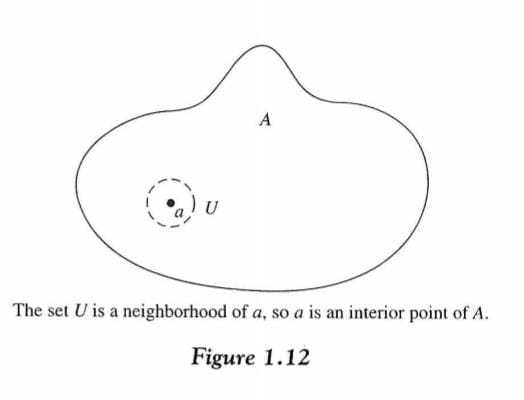
\includegraphics[width=3cm]{pembagian/Figure 1.12.jpg}
        \label{fig:enter-label}
    \end{figure}

    \end{tcolorbox}
Catatan:\\
Jika $A$ adalah subset dari ruang topologi ($\nX, \nT$) dan $B =$ \{$x \in \nX : x$ adalah titik interior dari $A$\}, maka $B =$ int($A$). Kemudian, jika ($\nX,d$) adalah ruang metrik, $A \subseteq \nX$ dan $x \in A $, maka $x$ $\in$ int($A$) jika dan hanya jika terdapat bilangan bulat positif $\epsilon$ sedemikian sehingga $B(x,\epsilon) \subseteq A$
\end{frame}

\begin{frame}{Teorema Interior}
    \begin{tcolorbox}[enhanced,title=Teorema 1.24, frame style tile={width=\paperwidth}{\wallpaper}]
        Misalkan $A$ dan $B$ adalah subset dari ruang topologi $(\nX, \nT)$, maka : 
        \begin{enumerate}
        \item $A$ buka jika dan hanya jika $A = int(A)$.
        \item Jika $A \subseteq B$ , maka $int(A) \subseteq int(B)$
        \item $int(A \cap B) = int($A$) \cap int(B)$
        \item $int(A) \cup int(B) \subseteq int(A \cup B)$
        \end{enumerate}
    \end{tcolorbox}
\end{frame}

\begin{frame}{Teorema Interior}
    \begin{tcolorbox}[enhanced,title=Teorema 1.24, frame style tile={width=\paperwidth}{\wallpaper}]
        1. Misalkan $A$ dan $B$ adalah subset dari ruang topologi ($\nX, \nT$), maka : \\
        $A$ buka jika dan hanya jika $A = int(A)$. \\

        Bukti : [Lihat Exercise 10]
        
    \end{tcolorbox}
\end{frame}

\begin{frame}{Teorema Interior}
    \begin{tcolorbox}[enhanced,title=Teorema 1.24, frame style tile={width=\paperwidth}{\wallpaper}]
        Misalkan $A$ dan $B$ adalah subset dari ruang topologi ($\nX, \nT$), maka : \\
        2. Jika $A \subseteq B$ , maka $int(A) \subseteq int(B)$ \\
        Bukti :
        \begin{itemize}
            \item Misalkan $A \subseteq B$, akan dibuktikan jika $x \in int(A)$ maka $x \in int (B)$
            \item Ambil sembarang $x \in int(A)$.
            \item Karena $x \in int(A)$, maka berdasarkan definisi, terdapat lingkungan U dari x sehingga $U \subseteq A$
            \item karena $U \subseteq A $ dan $A \subseteq B$, maka $U \subseteq B$ sehingga $x \in int (B)$
            \item Karena $x \in int (B)$, maka $int(A) \subseteq int(B)$
        \end{itemize}
    \end{tcolorbox}
\end{frame}

\begin{frame}{Teorema Interior}
    \begin{tcolorbox}[enhanced,title=Teorema 1.24, frame style tile={width=\paperwidth}{\wallpaper}]
        Misalkan $A$ dan $B$ adalah subset dari ruang topologi ($\nX, \nT$), maka : \\
        3. $int(A \cap B) = int(A) \cap int(B)$ \\

        Bukti : [Lihat Exercise 10]
        
    \end{tcolorbox}
\end{frame}

\begin{frame}{Teorema Interior}
    \begin{tcolorbox}[enhanced,title=Teorema 1.24, frame style tile={width=\paperwidth}{\wallpaper}]
        Misalkan $A$ dan $B$ adalah subset dari ruang topologi ($\nX, \nT$), maka : \\
        4. $int(A) \cup int(B) \subseteq int(A \cup B)$
    \end{tcolorbox}
\end{frame}

\begin{frame}{Teorema Interior}
    \begin{tcolorbox}[enhanced,title=Teorema 1.24, frame style tile={width=\paperwidth}{\wallpaper}]
        Bukti :
        \begin{itemize}
            \item Ambil sembarang $x \in int(A) \cup int(B)$. Akan dibuktikan $x \in int(A \cup B)$
            \item karena $x \in int(A) \cup int(B)$ maka $x \in int(A)$ atau $x \in int(B)$
            \item Karena $x \in int(A)$ maka berdasarkan definisi, terdapat lingkungan $U$ dari $x$ sehingga $U \subseteq A$
            \item Karena $x \in int(B)$ maka berdasarkan definisi, terdapat lingkungan $U$ dari $x$ sehingga $U \subseteq B$
            \item Pada kedua kasus, maka $U \subseteq A \cup B$, sehingga $x \in int(A \cup B)$ 
            \item Karena $x \in int(A \cup B)$ maka $int(A) \cup int(B) \subseteq int(A \cup B)$
        \end{itemize}
        
    \end{tcolorbox}
\end{frame}

\begin{frame}{Contoh 48}
    \begin{tcolorbox}[enhanced,title= Contoh 48, frame style tile={width=\paperwidth}{\wallpaper}]
        Misalkan $\nF$ adalah usual topologi di $\R$, misalkan juga $A$ = [$0, 1$] dan $B$ = [$1, 2$], Maka int($A \cup B$) = ($0,2$). Namun, int($A$) = ($0,1$) dan int($B$) = ($1,2$) sehingga $int($A$) \cup int(B) = (0,1) \cup (1,2)$

        
    \end{tcolorbox}
\end{frame}

\begin{frame}{Nowhere Dense}
    \begin{tcolorbox}[enhanced,title= Definisi, frame style tile={width=\paperwidth}{\wallpaper}]
        Suatu subset $A$ dari ruang topologi dikatakan \textbf{nowhere dense} jika memenuhi $int(\bar{A}) = \varnothing$
    \end{tcolorbox}
\end{frame}

\begin{frame}{Relative Discrete}
    \begin{tcolorbox}[enhanced,title= Definisi, frame style tile={width=\paperwidth}{\wallpaper}]
        Suatu subset $A$ dari ruang topologi ($\nX, \nT$) dikatakan \textbf{relatively discrete} jika untuk setiap $a \in A$, terdapat $U \in \nT$ sedemikian sehingga $U \cap A$ = \{$a$\}
    \end{tcolorbox}
\end{frame}

\begin{frame}{Teorema 1.25}
    \begin{tcolorbox}[enhanced,title= Teorema 1.25, frame style tile={width=\paperwidth}{\wallpaper}]
        Misalkan ($\nX, \nT$) adalah ruang topologi, Misalkan $C$ merupakan subset tutup dari $\nX$ dan misalkan $U$ adalah subset buka dari $\nX$, maka $C - U$ tutup dan $U - C$ Buka. \\
        Bukti : [Lihat Exercise 29]
    \end{tcolorbox}
\end{frame}

\begin{frame}{Teorema 1.26}
    \begin{tcolorbox}[enhanced,title= Teorema 1.26, frame style tile={width=\paperwidth}{\wallpaper}]
        Misalkan ($\nX, d$) adalah ruang metrik, Misalkan $x \in \nX$ dan misalkan $\epsilon$ dan $\delta$ adalah bilangan bulat positif yang memenuhi $\delta < \epsilon$, maka $\overline{B(x,\delta)} \subseteq B(x,\epsilon)$  \\
        Bukti : [Lihat Exercise 30]
    \end{tcolorbox}
\end{frame}

\begin{frame}{Perfect Set}
    \begin{tcolorbox}[enhanced,title= Definisi, frame style tile={width=\paperwidth}{\wallpaper}]
        Suatu Subset $A$ dari ruang topologi ($\nX, \nT$) dikatakan \textbf{perfect set} jika $A$ = $A'$  \\
    \end{tcolorbox}
\end{frame}

\begin{frame}{Isolated Point}
    \begin{tcolorbox}[enhanced,title= Definisi, frame style tile={width=\paperwidth}{\wallpaper}]
        Suatu titik $x$ dari subset A dari ruang topologi ($\nX, \nF$) dikatakan \textbf{isolated point} jika terdapat lingkungan $x$ yang tidak memuat titik $A$ yang berbeda dari $x$.

    \end{tcolorbox}
\end{frame}

\begin{frame}{Perfect Set}
    \begin{tcolorbox}[enhanced,title= Teorema 1.27, frame style tile={width=\paperwidth}{\wallpaper}]
        Suatu subset $A$ dari ruang topologi ($\nX, \nF$) dikatakan \textbf{perfect set} jika dan hanya jika subset tersebut tutup dan tidak punya \textbf{isolated point} \\
        Bukti : [Lihat Exercise 24]

    \end{tcolorbox}
\end{frame}